\documentclass[man]{apa6}
\usepackage{lmodern}
\usepackage{amssymb,amsmath}
\usepackage{ifxetex,ifluatex}
\usepackage{fixltx2e} % provides \textsubscript
\ifnum 0\ifxetex 1\fi\ifluatex 1\fi=0 % if pdftex
  \usepackage[T1]{fontenc}
  \usepackage[utf8]{inputenc}
\else % if luatex or xelatex
  \ifxetex
    \usepackage{mathspec}
  \else
    \usepackage{fontspec}
  \fi
  \defaultfontfeatures{Ligatures=TeX,Scale=MatchLowercase}
\fi
% use upquote if available, for straight quotes in verbatim environments
\IfFileExists{upquote.sty}{\usepackage{upquote}}{}
% use microtype if available
\IfFileExists{microtype.sty}{%
\usepackage{microtype}
\UseMicrotypeSet[protrusion]{basicmath} % disable protrusion for tt fonts
}{}
\usepackage{hyperref}
\hypersetup{unicode=true,
            pdftitle={Week 5 Lab 8},
            pdfauthor={Shaina Trevino, Maria Schweer-Collins, Alejandra Garcia Isaza, \& Jonathan Pedroza},
            pdfkeywords={Trains, Planes, Automobiles},
            pdfborder={0 0 0},
            breaklinks=true}
\urlstyle{same}  % don't use monospace font for urls
\usepackage{graphicx,grffile}
\makeatletter
\def\maxwidth{\ifdim\Gin@nat@width>\linewidth\linewidth\else\Gin@nat@width\fi}
\def\maxheight{\ifdim\Gin@nat@height>\textheight\textheight\else\Gin@nat@height\fi}
\makeatother
% Scale images if necessary, so that they will not overflow the page
% margins by default, and it is still possible to overwrite the defaults
% using explicit options in \includegraphics[width, height, ...]{}
\setkeys{Gin}{width=\maxwidth,height=\maxheight,keepaspectratio}
\IfFileExists{parskip.sty}{%
\usepackage{parskip}
}{% else
\setlength{\parindent}{0pt}
\setlength{\parskip}{6pt plus 2pt minus 1pt}
}
\setlength{\emergencystretch}{3em}  % prevent overfull lines
\providecommand{\tightlist}{%
  \setlength{\itemsep}{0pt}\setlength{\parskip}{0pt}}
\setcounter{secnumdepth}{0}
% Redefines (sub)paragraphs to behave more like sections
\ifx\paragraph\undefined\else
\let\oldparagraph\paragraph
\renewcommand{\paragraph}[1]{\oldparagraph{#1}\mbox{}}
\fi
\ifx\subparagraph\undefined\else
\let\oldsubparagraph\subparagraph
\renewcommand{\subparagraph}[1]{\oldsubparagraph{#1}\mbox{}}
\fi

%%% Use protect on footnotes to avoid problems with footnotes in titles
\let\rmarkdownfootnote\footnote%
\def\footnote{\protect\rmarkdownfootnote}


  \title{Week 5 Lab 8}
    \author{Shaina Trevino\textsuperscript{1}, Maria
Schweer-Collins\textsuperscript{1}, Alejandra Garcia
Isaza\textsuperscript{1}, \& Jonathan Pedroza\textsuperscript{1}}
    \date{}
  
\shorttitle{Wk5Lb8}
\affiliation{
\vspace{0.5cm}
\textsuperscript{1} University of Oregon}
\keywords{Trains, Planes, Automobiles}
\usepackage{csquotes}
\usepackage{upgreek}
\captionsetup{font=singlespacing,justification=justified}

\usepackage{longtable}
\usepackage{lscape}
\usepackage{multirow}
\usepackage{tabularx}
\usepackage[flushleft]{threeparttable}
\usepackage{threeparttablex}

\newenvironment{lltable}{\begin{landscape}\begin{center}\begin{ThreePartTable}}{\end{ThreePartTable}\end{center}\end{landscape}}

\makeatletter
\newcommand\LastLTentrywidth{1em}
\newlength\longtablewidth
\setlength{\longtablewidth}{1in}
\newcommand{\getlongtablewidth}{\begingroup \ifcsname LT@\roman{LT@tables}\endcsname \global\longtablewidth=0pt \renewcommand{\LT@entry}[2]{\global\advance\longtablewidth by ##2\relax\gdef\LastLTentrywidth{##2}}\@nameuse{LT@\roman{LT@tables}} \fi \endgroup}


\DeclareDelayedFloatFlavor{ThreePartTable}{table}
\DeclareDelayedFloatFlavor{lltable}{table}
\DeclareDelayedFloatFlavor*{longtable}{table}
\makeatletter
\renewcommand{\efloat@iwrite}[1]{\immediate\expandafter\protected@write\csname efloat@post#1\endcsname{}}
\makeatother

\authornote{

Correspondence concerning this article should be addressed to Shaina
Trevino, Postal address. E-mail:
\href{mailto:my@email.com}{\nolinkurl{my@email.com}}}

\abstract{
If You Have Two Loaves of Bread, Sell One and Buy a Lily - A Chinese
Proverb


}

\begin{document}
\maketitle

\section{Results}\label{results}

The table below presents the mean scores and standard deviations for
math and reading separated by sex(i.e., boys and girls) and whether
these students receive free/reduced price meals or not.

\begin{tabular}{l|l|r|r|r|r}
\hline
sex & frl & math\_mean & math\_sd & rdg\_mean & rdg\_sd\\
\hline
boy & no & 492.85 & 46.34 & 441.46 & 32.32\\
\hline
boy & yes & 469.87 & 46.09 & 425.38 & 26.63\\
\hline
girl & no & 501.21 & 45.96 & 448.54 & 34.52\\
\hline
girl & yes & 477.51 & 46.30 & 430.80 & 27.42\\
\hline
\end{tabular}

As shown in \emph{Figure 1} (at the end of the document), we observed a
slight positive association between the number of years of teaching
experience and students' math scores. Teachers who reported more years
of teaching experience were also more likely to have students in their
class with higher math scores, compared to teachers with less
experience. This association was present for both students who recieved
free and reduced meals and those who do not. However, the plot shows
that students who do receive free and reduced lunches, on average, had
lower math scores than students with paid meal status, regardless of the
years of teaching experience of their educator.

\begin{figure}
\centering
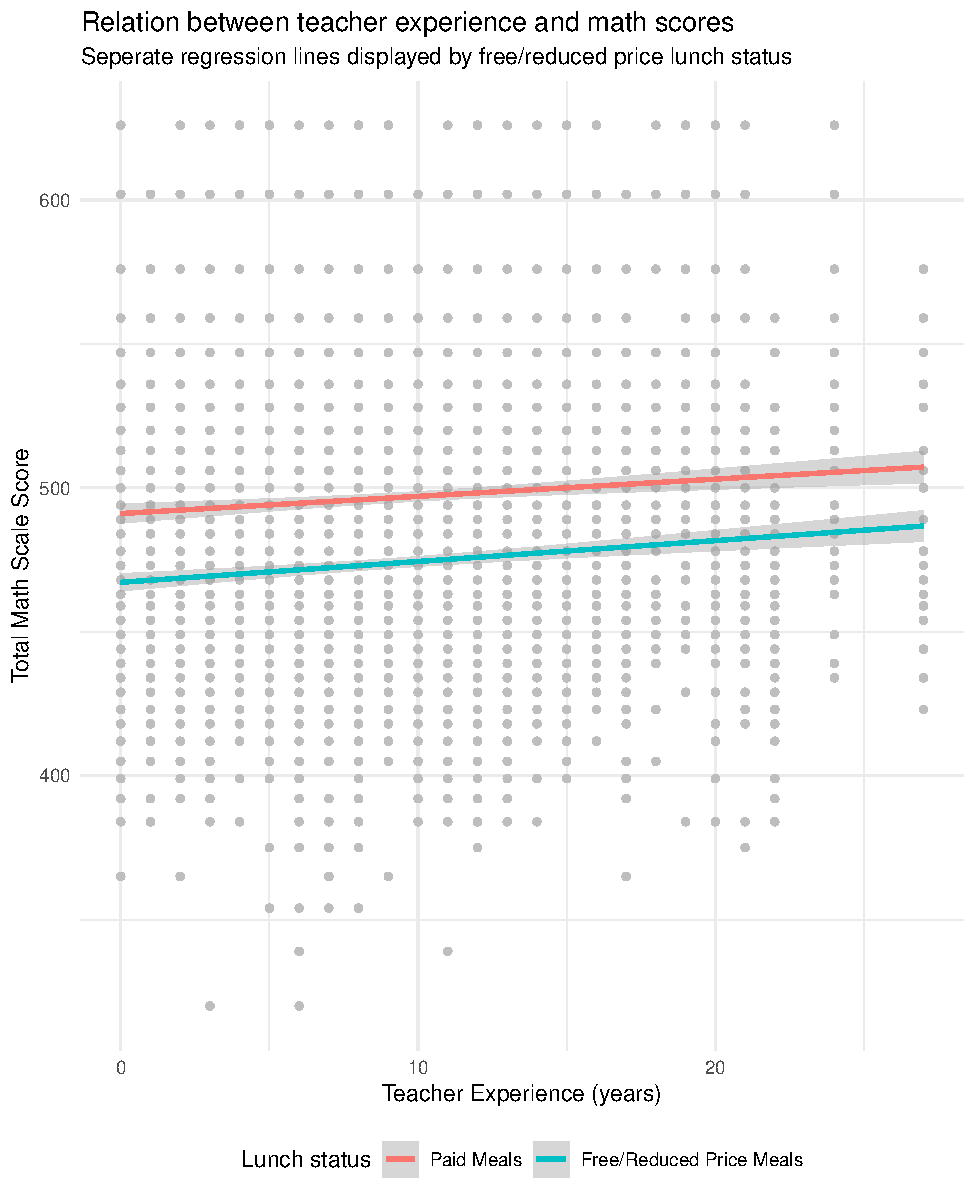
\includegraphics{Week_5_Lab_8_files/figure-latex/plot-1.pdf}
\caption{}
\end{figure}

\section{Discussion}\label{discussion}

Child maltreatment is characterized by its multifinality, this means
that individual differences play a role in how child maltreatment is
experienced and how it affects later development. In part, this can be
explained by timing, dose, chronicity and type of maltreatment (Gunnar,
Fisher, \& others, 2006). For instance, Cowell, Cicchetti, Rogosch \&
Toth (2015) found that on measures of inhibitory control and working
memory, maltreated children showed poorer performance than their
non-maltreated counterparts. Furthermore, Cowell et al. (2015) found
that within the maltreated group, children that had experienced
maltreatment during infancy had worse performance in comparison with
children that experienced maltreatment later in childhood.

\newpage

\section{References}\label{references}

\begingroup
\setlength{\parindent}{-0.5in} \setlength{\leftskip}{0.5in}

\hypertarget{refs}{}
\hypertarget{ref-cowell2015childhood}{}
Cowell, R. A., Cicchetti, D., Rogosch, F. A., \& Toth, S. L. (2015).
Childhood maltreatment and its effect on neurocognitive functioning:
Timing and chronicity matter. \emph{Development and Psychopathology},
\emph{27}(2), 521--533.

\hypertarget{ref-gunnar2006bringing}{}
Gunnar, M. R., Fisher, P. A., \& others. (2006). Bringing basic research
on early experience and stress neurobiology to bear on preventive
interventions for neglected and maltreated children. \emph{Development
and Psychopathology}, \emph{18}(3), 651--677.

\endgroup


\end{document}
